\chapter{Introducción}
\label{chapter:introduccion}


%%% SECTION
\section{Contexto y justificación del trabajo}

La polinización es un proceso crucial para la reproducción de muchas especies vegetales, incluyendo cultivos agrícolas de importancia económica, de hecho, tres cuartos (75\%) de los 111 cultivos agrícolas más importantes en todo el mundo dependen, en mayor o menor medida, de la polinización realizada por animales \cite{klein-2006}. 

Los polinizadores, como las abejas, mariposas, pájaros y murciélagos, desempeñan un papel esencial en la transferencia de polen de una flor a otra, permitiendo la fertilización y la producción de frutas y semillas. De todos estos animales, los insectos son los polinizadores más importantes, ya que son responsables de la polinización de más del 67\% de las especies de plantas con flores en todo el mundo \cite{innovatione-agrofood-design-2021}.

Sin embargo, en las últimas décadas, ha habido una disminución preocupante en la población de polinizadores debido a factores como la pérdida de hábitat, el uso de pesticidas y el cambio climático \cite{unam-2019}. Esto plantea una amenaza significativa para la seguridad alimentaria y la biodiversidad global.

Para abordar esta problemática, es crucial comprender y monitorear la actividad de los polinizadores en diferentes entornos. La observación directa y el seguimiento manual de los polinizadores pueden ser costosos y laboriosos. Aquí es donde entra en juego la tecnología de visión por computadora y las redes neuronales convolucionales.

La detección de polinizadores a partir de imágenes utilizando redes neuronales convolucionales ofrece numerosos beneficios como por ejemplo:

\begin{itemize}
    \item 
    \textbf{Eficiencia y Escalabilidad:} Las redes neuronales convolucionales permiten procesar grandes conjuntos de datos de imágenes de manera eficiente y automatizada. Esto significa que es posible recolectar y analizar todas las interacciones en una cantidad significativa de datos en un corto período de tiempo, lo que facilita la monitorización a largo plazo.
    
    \item 
    \textbf{Precisión:} Las CNN son conocidas por su capacidad para detectar patrones y características en imágenes con alta precisión. Esto garantiza que las detecciones de polinizadores sean confiables y consistentes.
    
    \item 
    \textbf{Aplicabilidad:} Este enfoque puede ser aplicado en una variedad de entornos, desde campos agrícolas hasta áreas naturales, lo que lo hace relevante tanto para la investigación científica como para la toma de decisiones en agricultura y conservación.
\end{itemize}

El objetivo de este trabajo es utilizar redes neuronales convolucionales para construir un modelo que habilite la detección de polinizadores y los clasifique en grupos funcionales, con lo que se pueda reconstruir una red de polinización. De esta manera, se podrá monitorear la actividad de los polinizadores en diferentes entornos y se podrá identificar tendencias en las poblaciones de polinizadores. Esto brindará información valiosa para las instituciones de investigación como para los diferentes departamentos gubernamentales y no gubernamentales en la toma de decisiones para la agricultura y la conservación.



\section{Motivación}

Mi trayectoria como docente e investigador en la Facultad de Ciencias Exactas y Naturales de la Pontificia Universidad Católica del Ecuador se ha enriquecido significativamente gracias a la colaboración interdisciplinaria con colegas de la Escuela de Biología. Estas sinergias han abierto oportunidades únicas para integrar mi especialización en matemáticas y ciencia de datos con el estudio y la preservación de la biodiversidad ecuatoriana, un campo de vital importancia en un país que se distingue por ser el sexto más megadiverso del mundo.

La interacción con estas diversas disciplinas me ha permitido acompañar a estudiantes tanto de Biología como de Ciencia de Datos en salidas de campo, donde la teoría se encuentra con la práctica. Estas experiencias en el terreno han sido fundamentales para comprender la complejidad y la riqueza de las especies de nuestro país, muchas de las cuales aún están por descubrir. Esta inmersión directa en el estudio de la biodiversidad ha fortalecido mi convicción de que la conservación efectiva requiere de enfoques innovadores y técnicas avanzadas, como el reconocimiento automático de imágenes, para enfrentar los desafíos emergentes como la deforestación, la caza furtiva, la contaminación y el cambio climático.

A través de este trabajo, se busca contribuir con un enfoque que permita la reconstrucción de redes de polinización de manera más eficiente y no invasiva. La meta es proporcionar herramientas que mejoren nuestra capacidad de monitoreo y protección de las especies, particularmente en extensas áreas donde la aparición de nuevas especies requiere una rápida inclusión en los planes de conservación. Este proyecto representa la confluencia de mi experiencia en el aula y en el campo, mi colaboración con expertos en Biología y mi formación en Ciencia de Datos, todo dirigido hacia un objetivo común: proteger y entender mejor el tesoro natural que Ecuador posee.

\section{Objetivos}

\subsection{Objetivo principal}

Construir y entrenar una red neuronal convolucional para la detección de polinizadores en imágenes de flores, que sirva de manera universal para la reconstrucción de redes de polinización. 

\subsection{Objetivos específicos}

\begin{itemize}
    \item Depurar un conjunto de datos de imágenes de polinizadores.
    \item Seleccionar un modelo de red neuronal convolucional para la detección de polinizadores en imágenes.
    \item Entrenar la red neuronal convolucional sobre el conjunto de datos de imágenes de polinizadores construida.
    \item Reconstruir una red de polinización a partir de las detecciones de la red neuronal convolucional.
    \item Evaluar los resultados analizando las métricas de la red de polinizadores reconstruida.
\end{itemize}

\section{Metodología}

Como es usual en los proyectos de Ciencia de Datos, el proyecto se divide en las siguientes etapas: recopilación y preparación de datos, creación de modelo a aplicarse sobre los datos y evaluación contextualizada de los resultados obtenidos.

En lo que respecta a la recopilación y preparación de datos, se utilizará un conjunto de alrededor de cinco mil imágenes (5000) registradas en dos hábitats y cuatro lugares de estudio en Cabrera (Islas Baleares, ver Figura \ref{fig:ubicacion}). Los polinizadores están identificados por expertos y etiquetados utilizando las siguientes categorías: «Bee», «Diptera», «Coleoptera», «Hoverfly», «Lepidoptera», «Wasp» y «Others». 

\begin{figure}[H]
    \centering
    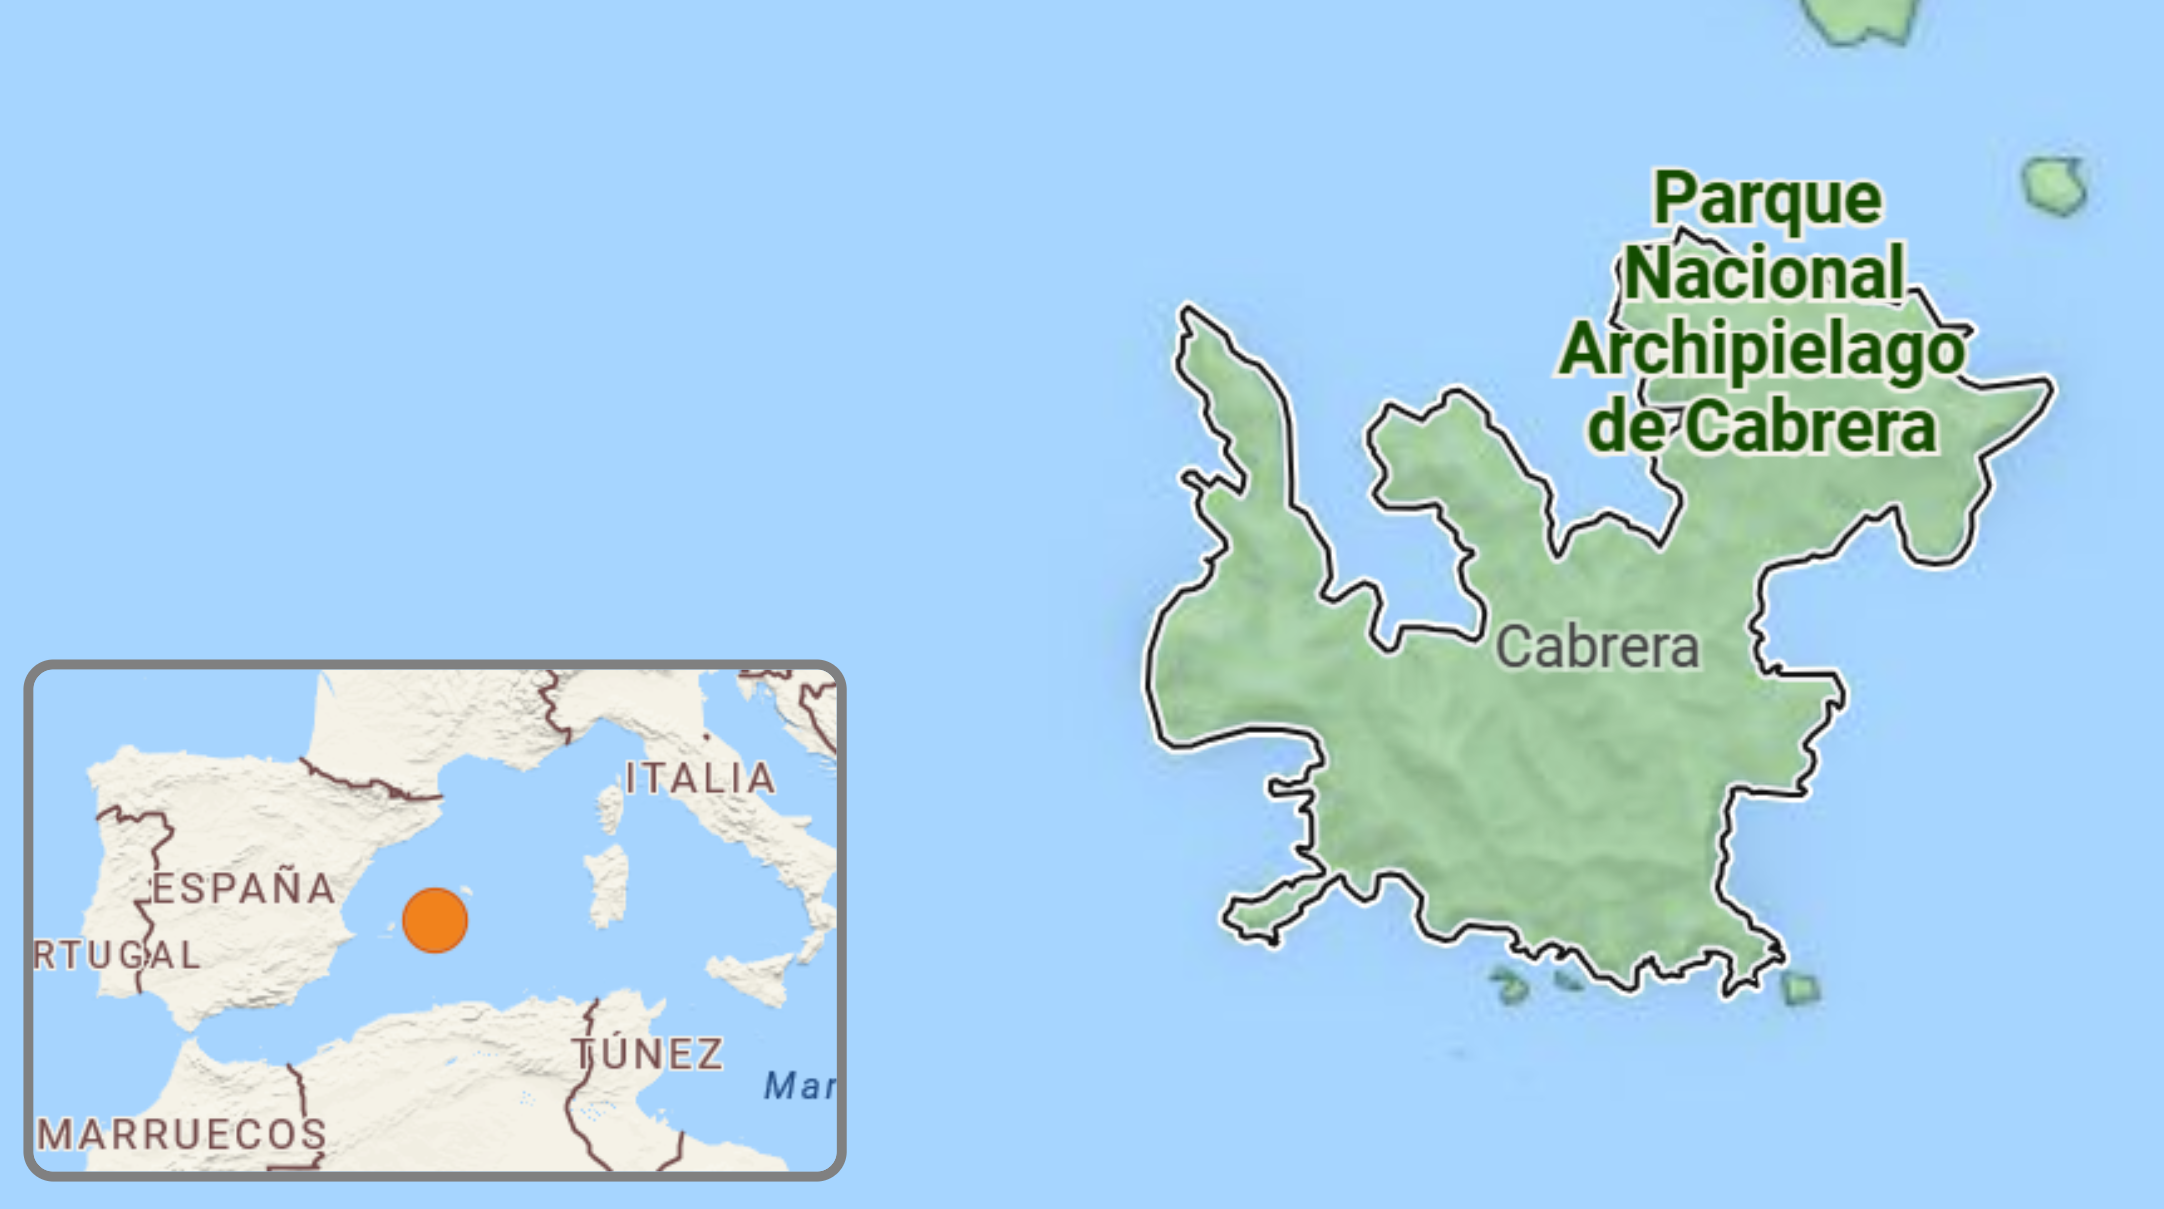
\includegraphics[width=0.9\textwidth]{Figuras/ubicacion.png}
    \caption[Ubicación de Cabrera.]{Ubicación de Cabrera. Tomado de Bing \cite{bing_maps}}
    \label{fig:ubicacion}
\end{figure}

Para realizar la identificación de las plantas que se hallan en el fondo de las imágenes, se utilizará la herramienta \textit{My PlantNet API} \cite{PlantNet}. Se planteará la identificación a nivel de Familia, para, de esta manera, obtener los grupos de plantas que cada insecto poliniza.

Esta será la etapa de partida para la construcción del conjunto de datos de imágenes de polinizadores que será utilizado para el entrenamiento y evaluación de las etapas posteriores. Finalmente, de darse el caso, se utilizarán técnicas tradicionales de aumento de imágenes para incrementar el tamaño del conjunto de datos; entre estas, se encuentran la rotación, el recorte, el volteo, el cambio de color, etc.


Por el lado del diseño de una red neuronal convolucional para la detección de polinizadores en imágenes, se analizarán dos alternativas: la arquitectura de red neuronal convolucional \textit{YOLOv5}  que ha demostrado dar buenos resultados en la detección de objetos en imágenes, en especial, de insectos \cite{ahmad-2022,qi-2023}; y la arquitectura de red neuronal convolucional \textit{EfficientNET} que ha obtenido resultados de precisión altos cuando se trata de pocas clases \cite{monis-2022}.

En lo relacionado con la evaluación contextualizada de los resultados obtenidos, en primera instancia, se utilizarán las métricas de precisión, sensibilidad y especificidad para evaluar el desempeño de la red neuronal convolucional. Además, a partir de los resultados, se reconstruirá una red de polinización bajo la metodología descrita en \cite{young-2021} y se analizarán las métricas de la misma.

Finalmente, en lo que respecta a la documentación del proyecto, se utilizará el lenguaje de programación Python y el entorno de desarrollo Jupyter Notebook. En específico, se utilizará la librería \textit{Tensorflow} y \textit{Pytorch} para la construcción de la red neuronal convolucional y la librería \textit{NetworkX} para el análisis y visualización de la red de polinización. El código fuente del proyecto se encontrará disponible en el repositorio de GitHub (ver Anexo \ref{anexo:github}). Adicionalmente, los pesos de los modelos entrenados se encontrarán disponibles en el repositorio particular de OneDrive del autor (ver Anexo \ref{anexo:pesos}).

\section{Planificación}

En la Figura \ref{fig:plan} se muestra el diagrama Gantt de la propuesta de planificación de las diferentes actividades del proyecto.

Las actividades del proyecto se agrupan en cuatro etapas: Definición y planificación del trabajo, Elaboración del estado del arte, Diseño e implementación del trabajo, Redacción de la memoria. Adicionalmente, se incluye una etapa de Defensa del trabajo.

Para la primera etapa, se estima una duración de 2 semanas. En esta etapa se realizará la definición de la propuesta, los objetivos y la metodología. Para la segunda etapa, se estima una duración de 3 semanas. En esta etapa se realizará la recolección de información y la redacción del estado del arte. Para la tercera etapa, se estima una duración de 8 semanas. En esta etapa se realizará la construcción del conjunto de datos, el diseño de la red neuronal, el entrenamiento de la red neuronal y la reconstrucción de la red de polinización; se finaliza con la evaluación de los resultados. Para la cuarta etapa, se estima una duración de 4 semanas. En esta etapa se realizará la redacción de la memoria. Finalmente, para la quinta etapa, se estima una duración de 1 semana. En esta etapa se realizará la defensa del trabajo.

De manera específica, en la Figura \ref{fig:plan} se aprecian la distribución de las actividades en el tiempo. Los rombos representas las fechas de entrega de avances del proyecto.

\begin{figure}[H]
    \centering
    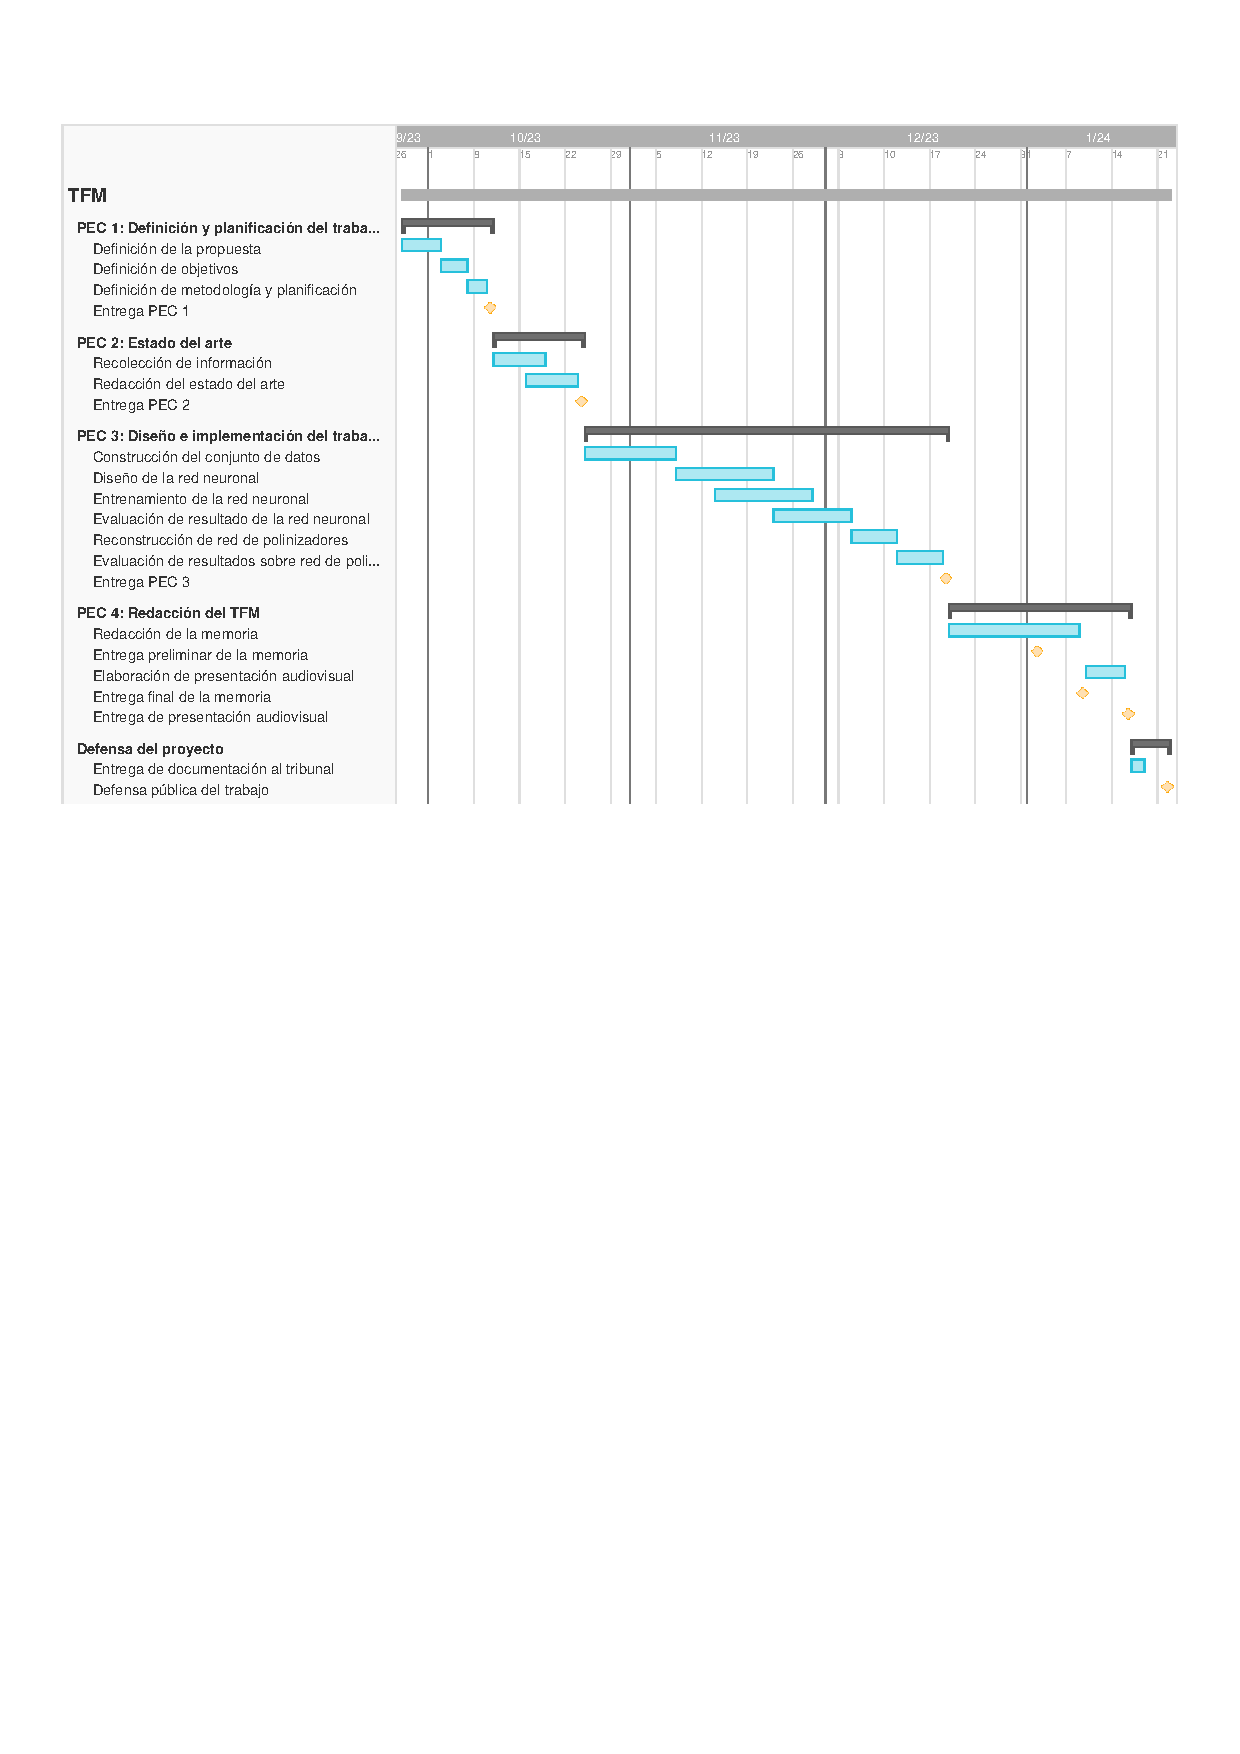
\includegraphics[width=1.44\textwidth,angle=90]{Figuras/PlanTFM.pdf}
    \caption{Diagrama Gantt de la planificación del proyecto.}
    \label{fig:plan}
\end{figure}


\section{Impacto en sostenibilidad, ético-social y de diversidad}

\paragraph{Sostenibilidad:} Este proyecto contribuye al ODS 15 (Vida de Ecosistemas Terrestres), ya que promueve la sostenibilidad de los ecosistemas terrestres. Al facilitar la monitorización y el estudio de los polinizadores, contribuye a la conservación de la biodiversidad y al mantenimiento de ecosistemas saludables, esenciales para la seguridad alimentaria y el equilibrio natural. Además, al emplear tecnologías de visión por computadora, reduce la necesidad de métodos de monitoreo invasivos y laboriosos, alineándose con prácticas sostenibles y de bajo impacto ambiental.

\paragraph{Comportamiento Ético y Responsabilidad Social:} Al mejorar la gestión de ecosistemas de polinizadores, este trabajo apoya indirectamente el ODS 2 (Hambre cero). Una identificación precisa de los polinizadores puede impulsar estrategias para optimizar prácticas agrícolas, aumentando la eficiencia de la polinización y mejorando los rendimientos de cultivos. Esto no solo fortalece la seguridad alimentaria, sino que también apoya prácticas agrícolas más éticas y sostenibles, contribuyendo al bienestar de las comunidades dependientes de la agricultura.

\paragraph{Diversidad, Género y Derechos Humanos:} Este proyecto contribuye al ODS 10 (Reducción de las desigualdades). La implementación de tecnologías de detección automática de polinizadores permite a países con recursos limitados acceder a información vital para la conservación de sus ecosistemas, equiparando su capacidad de cuidado y estudio de la biodiversidad con la de países de mayores recursos. Esto promueve una distribución más equitativa del conocimiento y las herramientas necesarias para la protección ambiental global.